%!TEX program = xelatex
%!TEX options = --shell-escape

\documentclass[table, 14pt, aspectratio=169]{beamer}

\setbeamerfont{title}{series=\bfseries}
\setbeamerfont{frametitle}{series=\bfseries}
\usefonttheme[onlymath]{serif}

\definecolor{OxfordBlue}{RGB}{0, 33, 71}
\definecolor{OxfordGoldPale}{RGB}{243,222,116}
\setbeamercolor{title}{fg=OxfordBlue}
\setbeamercolor{frametitle}{fg=OxfordBlue}
\setbeamercolor{section in toc}{fg=black}
\setbeamercolor{description item}{fg=black}
\setbeamertemplate{description item}{\bfseries\insertdescriptionitem}
\setbeamercolor{local structure}{fg=OxfordBlue}
\setbeamertemplate{itemize item}{\color{OxfordBlue}$\blacktriangleright$}
\setbeamertemplate{itemize subitem}{\color{OxfordBlue}$\blacktriangleright$}
\setbeamertemplate{itemize subsubitem}{\color{OxfordBlue}$\blacktriangleright$}
\setbeamerfont{block title}{series=\bfseries}
\setbeamercolor{block title}{use={frametitle},fg=frametitle.fg,bg=frametitle.bg}

\AtBeginSection[]{
  \begin{frame}
    \vfill\centering\usebeamerfont{title}\insertsectionhead\par\vfill
  \end{frame}
}

\newcommand{\hl}[1]{\textcolor{OxfordBlue}{\textbf{#1}}}

\usepackage{fontspec}
\setmonofont[Scale=MatchUppercase]{Fira Mono}
\setsansfont{FoundrySterling}[UprightFont=*-Book, BoldFont=*-Demi, ItalicFont=*-BookItalic]

\usetheme{default}
\beamertemplatenavigationsymbolsempty

\usepackage{changepage}

\newcommand{\tthl}[1]{\texttt{\hl{#1}}}

\usepackage[cache=false]{minted}
\usemintedstyle{NetLogo} % get it from http://netlogo-pygment.sourceforge.net/
\RecustomVerbatimEnvironment{Verbatim}{BVerbatim}{}
\newminted[nlogo]{nlogo}{autogobble}
\setminted{highlightcolor=OxfordGoldPale}
\usepackage{xparse}
\DeclareDocumentCommand \nlc { v } {\strut\mintinline[gobble=1]{nlogo}{ #1}}

\usepackage{tikz}
\usetikzlibrary{positioning, decorations.pathreplacing, fit, calligraphy, arrows.meta, backgrounds, shapes.callouts, shadows.blur}
\usepackage[export]{adjustbox}

\usepackage{hanging}

\usepackage{tcolorbox}
\tcbset{%
  noparskip,
  boxrule=0.25pt,
  colback=OxfordBlue!10, %background color of the box
  colframe=OxfordBlue!75!black, %color of frame and title background
  coltext=black, %color of body text
  coltitle=black, %color of title text
  fonttitle=\bfseries,
}

\usepackage{textpos}

\title{ABM and environmental policy}
\subtitle{A mini-Poseidon model in NetLogo}

\author{Nicolas Payette}
\institute{%
  
\includegraphics[height=2cm]{images/cohesys_logo_light_oxford.pdf}
}

\begin{document}

\begin{frame}
  \titlepage
\end{frame}

\begin{frame}{What's the plan?}
  \large
  \begin{itemize}
    \addtolength{\itemsep}{1ex}
    \item A little bit about the \hl{Poseidon} fisheries ABM
    \item A whole lot about building \hl{Poseidon in NetLogo}!
  \end{itemize}
\end{frame}

\begin{frame}{Why model fisheries?}
    
  \begin{itemize}
    \item It's big!
      \begin{itemize}
        \item 96.4 million tonnes of fish caught in 2018
        \item employing 59.51 million people
        \item 17\% of total animal protein consumed globally
      \end{itemize}
    \vfill
    \item It's in trouble!
      \begin{itemize}
        \item 34.2\% of stocks are overfished
      \end{itemize}
  \end{itemize}
  \vfill
  \hl{Why use ABM to do it?}
  \begin{itemize}
    \item They're inherently spatial;
    \item they involve complex interactions,
    \item between smart, adaptive agents.
  \end{itemize}
  \vfill
  \tiny Source: \url{http://www.fao.org/3/ca9231en/CA9231EN.pdf}
\end{frame}

\begin{frame}
  \begin{columns}[T]
    \begin{column}{0.35\textwidth}
      \Large\hl{Poseidon}
      \vskip 1ex
      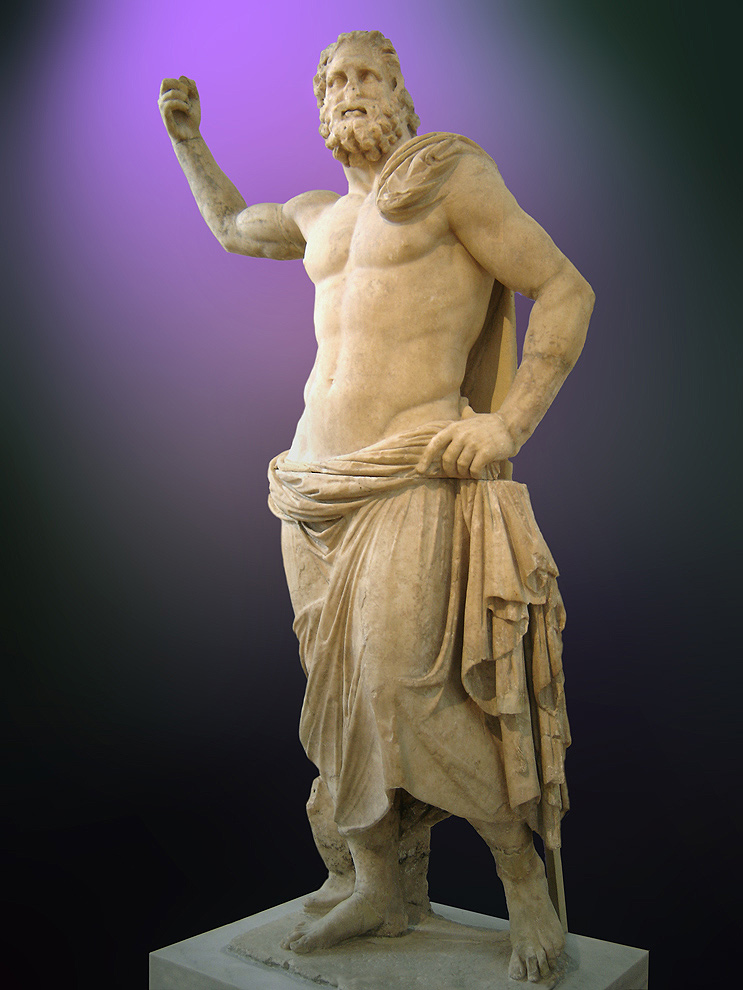
\includegraphics[width=\linewidth]{images/0036MAN_Poseidon}
      \tiny Source: Ricardo André Frantz, \url{https://w.wiki/wzx}
    \end{column}
    \begin{column}{0.65\textwidth}
      \hfill
      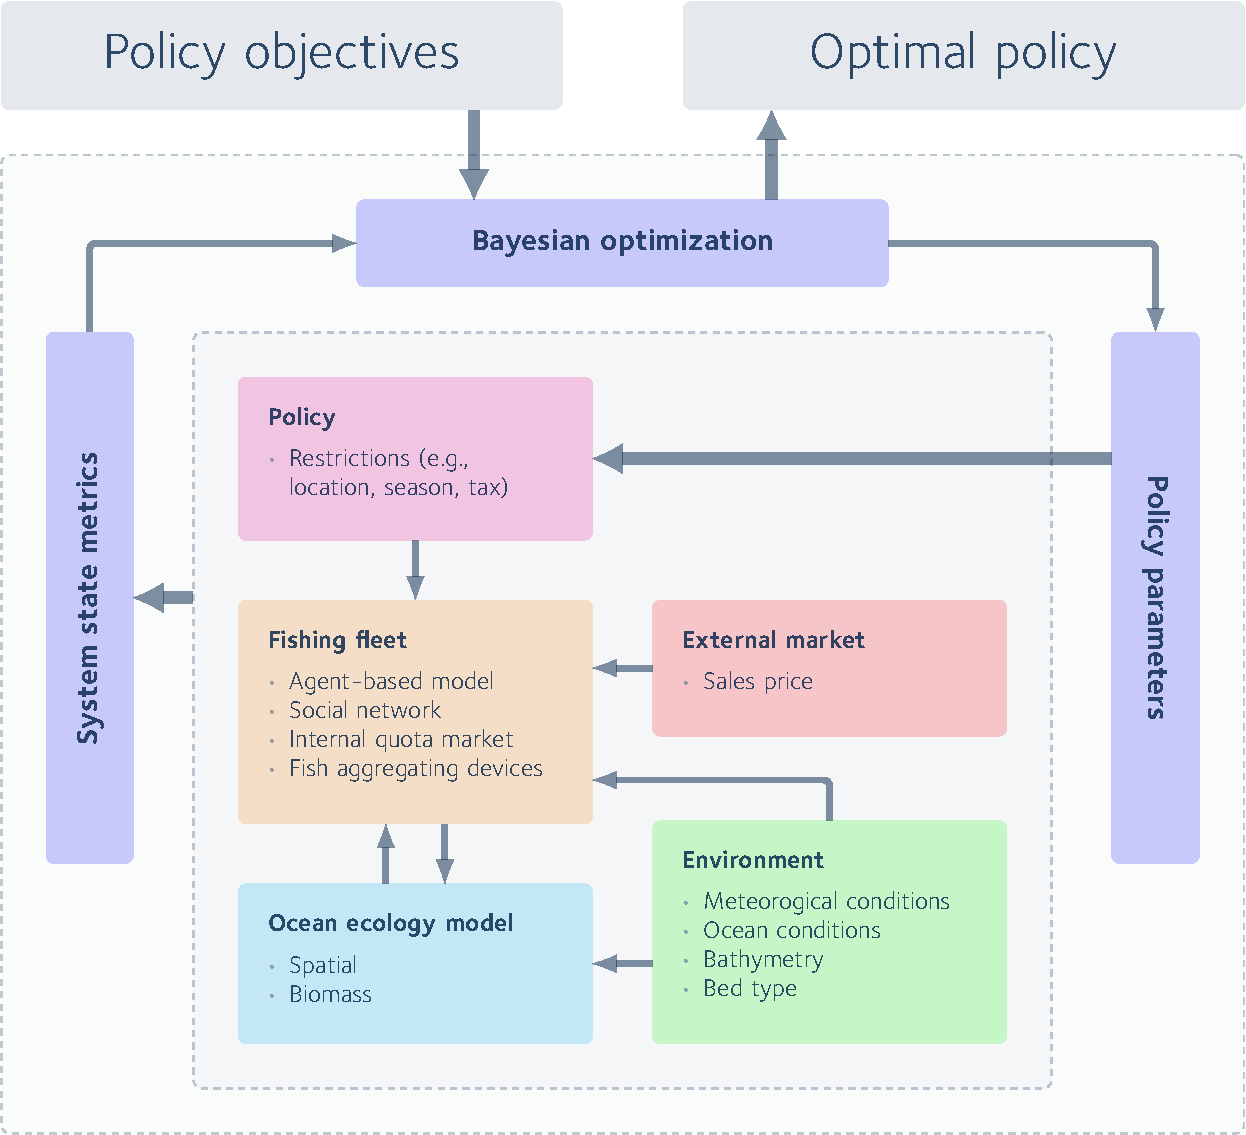
\includegraphics[height=0.95\textheight]{images/poseidon_diagram.pdf}
    \end{column}    
  \end{columns}
\end{frame}

\begin{frame}[t]\frametitle{Poseidon applications}
  \begin{columns}[T]
    \begin{column}{0.575\textwidth}
      \footnotesize
      \begin{itemize}
        \item Conceptual models
        \item US West Coast Groundfish
        \item Indonesian Deep water snapper grouper fishery
        \item Eastern Pacific Tuna Management
      \end{itemize}
      \vskip 1em
      
\includegraphics[width=\linewidth]{images/Design-Partners.png}
    \end{column}
    \begin{column}{0.425\textwidth}
      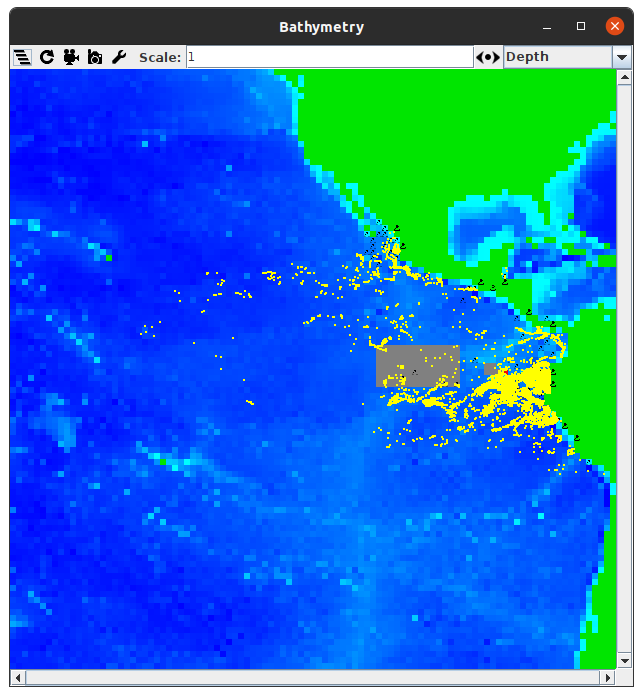
\includegraphics[width=\linewidth]{images/poseidon_screenshot.png}
    \end{column}
  \end{columns}
\end{frame}


\begin{frame}[t]\frametitle{What can we put in a minimal fisheries model?}
  \Large
  \vfill
  \begin{columns}[T]
    \begin{column}{0.3\textwidth}
      \hl{Agents:}
      \begin{itemize}
        \item A port,
        \item fishers,
        \item and fish!
      \end{itemize}
    \end{column}
    \begin{column}{0.6\textwidth}
      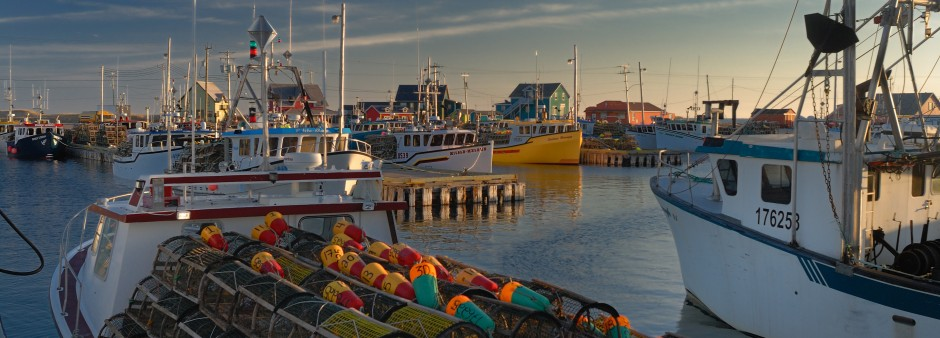
\includegraphics[width=\textwidth]{images/port.jpg}\\
      \tiny Source: \url{https://www.tourismeilesdelamadeleine.com/fr/decouvrir-les-iles/les-iles/ile-de-grande-entree}
    \end{column}
  \end{columns}
  \vfill
      \hl{Some policy to test:}
      \begin{itemize}
        \item The size of a marine protected area (MPA)
      \end{itemize}
\end{frame}

\begin{frame}[t]
  \Large Fisher agents in Poseidon use the\\\hl{``Explore, exploit, imitate''}\\behaviour algorithm:
  \vfill
  \begin{tcolorbox}[halign=flush left]
  \begin{itemize}\small
    \item Should I go exploring?
    \begin{itemize}\small
      \item If yes, pick a random spot not too far from my favourite spot (\hl{EXPLORE})
      \item If not, pick a friend and ask: is my favourite spot better than my friend's favourite spot?
      \begin{itemize}\small
        \item If it is, go to my favourite spot (\hl{EXPLOIT})
        \item If it isn't, go to my friend's favourite spot (\hl{IMITATE})
      \end{itemize}
    \end{itemize}
    \item If the spot I went to was better than my favourite spot, it becomes my new favourite!
  \end{itemize}
  \end{tcolorbox}
\end{frame}

\begin{frame}[t]\frametitle{A bit of biology}
  \begin{columns}
    \begin{column}{0.7\textwidth}
      {\small We do not simulate individual fish. We keep track of the total biomass and apply yearly \hl{logistic growth}.}
      $$\frac{dP}{dt}=r P \left(1 - \frac{P}{K}\right)$$
      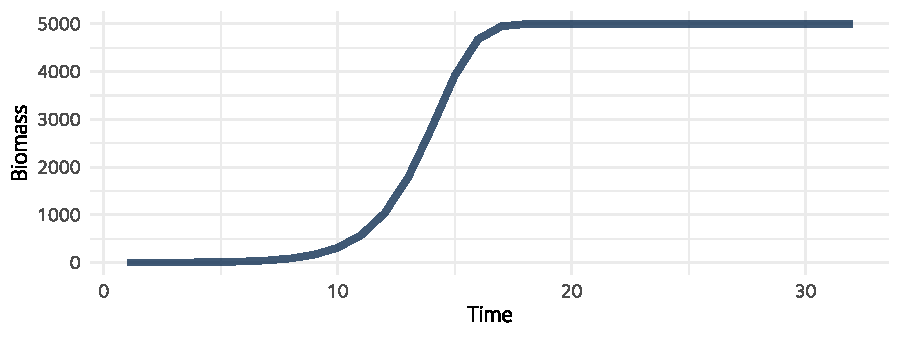
\includegraphics[width=\linewidth]{images/logistic_growth.pdf}
    \end{column}
    \begin{column}{0.3\textwidth}
      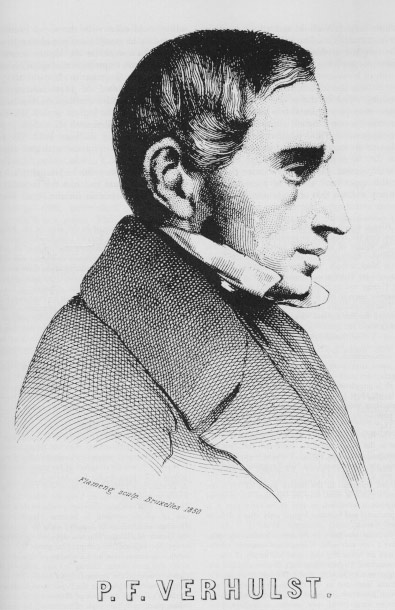
\includegraphics[width=\linewidth]{images/Pierre_Francois_Verhulst.jpg}\\
      \tiny Pierre-François Verhulst (1804--1849).\\Source: \url{https://w.wiki/x2o}.
    \end{column}
  \end{columns}

\end{frame}

\begin{frame}[fragile=singleslide]{Get the model skeleton from GitHub}
  \Large
  \centering
  \vfill
  \url{https://github.com/nicolaspayette/mini-poseidon}
  \vfill
\end{frame}

\begin{frame}[fragile=singleslide]\frametitle{Recoloring patches}
  \centering
  \begin{adjustbox}{max width=\linewidth}
    \begin{nlogo}
to recolor-patches
  ask patches [
    set pcolor scale-color blue (biomass / 2) carrying-capacity 0
  ]
end
    \end{nlogo}
  \end{adjustbox}
  \vfill
  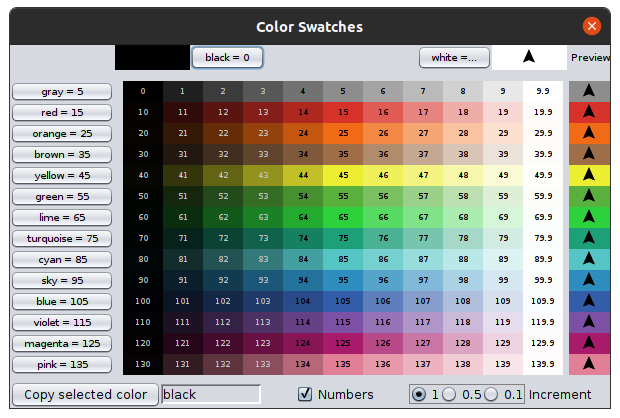
\includegraphics[width=0.7\textheight]{images/swatches.png}
\end{frame}

\begin{frame}[fragile=singleslide]{Explore, exploit, imitate\ldots}\small
  \begin{adjustbox}{max height=0.8\textheight, max width = \linewidth}
    \begin{minted}{nlogo}
to pick-destination ; fisher procedure
  ifelse random-float 1 < exploration-probability [
    ; explore:
    let r 1 + random-poisson exploration-radius
    set trip-destination [ one-of fishable-patches in-radius r ] of favourite-destination
  ] [
    let other-fisher one-of other fishers
    let their-profits [ profits-at-favourite-destination ] of other-fisher
    ifelse profits-at-favourite-destination >= their-profits [
      ; exploit:
      set trip-destination favourite-destination
    ] [
      ; imitate
      set trip-destination [ favourite-destination ] of other-fisher
    ]
  ]
  set current-destination trip-destination
end
    \end{minted}  
  \end{adjustbox}
\end{frame}


\begin{frame}[fragile=singleslide]{Let's \texttt{go}!}
  \begin{adjustbox}{max height=0.8\textheight, max width = \linewidth}
    \begin{minted}[]{nlogo}
to go
  ask fishers [
    set trip-costs trip-costs + hourly-costs
    ifelse patch-here = current-destination [
      ifelse any? ports-here [ dock ] [ fish ]
    ] [
      face current-destination
      forward speed
    ]
  ]
  update-biology
  tick
end
    \end{minted}
  \end{adjustbox}
\end{frame}

\begin{frame}[fragile=singleslide]{Fishing!}
  \begin{adjustbox}{max height=0.8\textheight, max width = \linewidth}
    \begin{minted}[]{nlogo}
to fish ; fisher procedure
  set pcolor red
  let biomass-caught biomass * catchability
  set biomass biomass - biomass-caught
  set biomass-in-hold biomass-in-hold + biomass-caught
  set current-destination [ patch-here ] of one-of ports
end
    \end{minted}
  \end{adjustbox}
\end{frame}

\begin{frame}[fragile=singleslide]{Docking at the port}
  \begin{adjustbox}{max height=0.8\textheight, max width = \linewidth}
    \begin{minted}[]{nlogo}
to dock ; fisher procedure
  let revenues biomass-in-hold * price-of-fish
  set biomass-in-hold 0
  let profits revenues - trip-costs
  set trip-costs 0
  set bank-balance bank-balance + profits
  (ifelse
    trip-destination = favourite-destination [
      set profits-at-favourite-destination profits
    ]
    profits > profits-at-favourite-destination [
      set favourite-destination trip-destination
      set profits-at-favourite-destination profits
    ]
  )
  pick-destination
end
    \end{minted}
  \end{adjustbox}
\end{frame}


\begin{frame}[fragile=singleslide]{Updating the biology}
  \vfill
  $$\frac{dP}{dt}=r P \left(1 - \frac{P}{K}\right)$$
  \vfill
  \begin{adjustbox}{max width=\linewidth}
    \begin{nlogo}
to update-biology
  diffuse biomass diffusion-rate
  recolor-patches
  if ticks mod (15 * 24) = 0 [ ; every 15 days
    ask patches [
      set biomass biomass + (
        growth-rate * biomass * (1 - (biomass / carrying-capacity))
      )
    ]
  ]
end
    \end{nlogo}
  \end{adjustbox}
\end{frame}

\begin{frame}[fragile=singleslide]{Adding a protected area after one year}
  \begin{adjustbox}{max height=0.8\textheight, max width = \linewidth}
    \begin{minted}[]{nlogo}
to setup-mpa
  set-default-shape xs "x"
  ask patches with [ 
    pxcor >= min-mpa-x and 
    pxcor <= max-mpa-x and 
    pycor >= min-mpa-y and
    pycor <= max-mpa-y and
    not any? ports-here
  ] [
    sprout-xs 1 [ set color [ 0 0 0 50 ] ]
  ]
  set fishable-patches fishable-patches with [ not any? xs-here ]
end
    \end{minted}
  \end{adjustbox}
\end{frame}

\begin{frame}[fragile=singleslide]{Modify \texttt{go}}
  \begin{adjustbox}{max height=0.8\textheight, max width = \linewidth}
    \begin{minted}[highlightlines=2]{nlogo}
to go
  if ticks = 365 * 24 [ setup-mpa ]
  ask fishers [
    set trip-costs trip-costs + hourly-costs
    ifelse patch-here = current-destination [
      ifelse any? ports-here [ dock ] [ fish ]
    ] [
      face current-destination
      forward speed
    ]
  ]
  update-biology
  tick
end
    \end{minted}
  \end{adjustbox}
\end{frame}

\begin{frame}[fragile=singleslide]{Modify \texttt{dock}}
  %\begin{adjustbox}{max height=0.8\textheight, max width = \linewidth}
    \scriptsize
    \begin{minted}[highlightlines=16-20]{nlogo}
to dock ; fisher procedure
  let revenues biomass-in-hold * price-of-fish
  set biomass-in-hold 0
  let profits revenues - trip-costs
  set trip-costs 0
  set bank-balance bank-balance + profits
  (ifelse
    trip-destination = favourite-destination [
      set profits-at-favourite-destination profits
    ]
    profits > profits-at-favourite-destination [
      set favourite-destination trip-destination
      set profits-at-favourite-destination profits
    ]
  )
  if [ any? xs-here ] of favourite-destination [
    set favourite-destination min-one-of fishable-patches [ 
      distance [ favourite-destination ] of myself
    ]
  ]
  pick-destination
end
    \end{minted}
  %\end{adjustbox}
\end{frame}

\begin{frame}[fragile=singleslide]{Figuring out the bottlenecks in our model}
  \begin{adjustbox}{max height=0.8\textheight, max width = \linewidth}
    \begin{minted}{nlogo}  
to profile
  setup                                          
  profiler:start                                 
  repeat 365 * 24 * 4 [ go ]                      
  profiler:stop     
  print profiler:report         
  csv:to-file "profiler_data.csv" profiler:data  
  profiler:reset                                 
end
    \end{minted}
  \end{adjustbox}
\end{frame}

\begin{frame}{Scenario}
  \vfill
  We have observed the real-world fishery for one year.
  \vfill
  Fishers ended up with a mean bank balance of £775,000.
  \vfill
  We want to:
  \vfill
  \begin{itemize}
    \item Use this information to estimate the EEI algorithm parameters.
    \vfill
    \item Simulate the fishery for three more years under the ``business as usual'' scenario.
    \vfill
    \item Figure out the best location for an MPA.
  \end{itemize}
  \vfill
\end{frame}

\begin{frame}{Estimating EEI parameters}
  \centering
  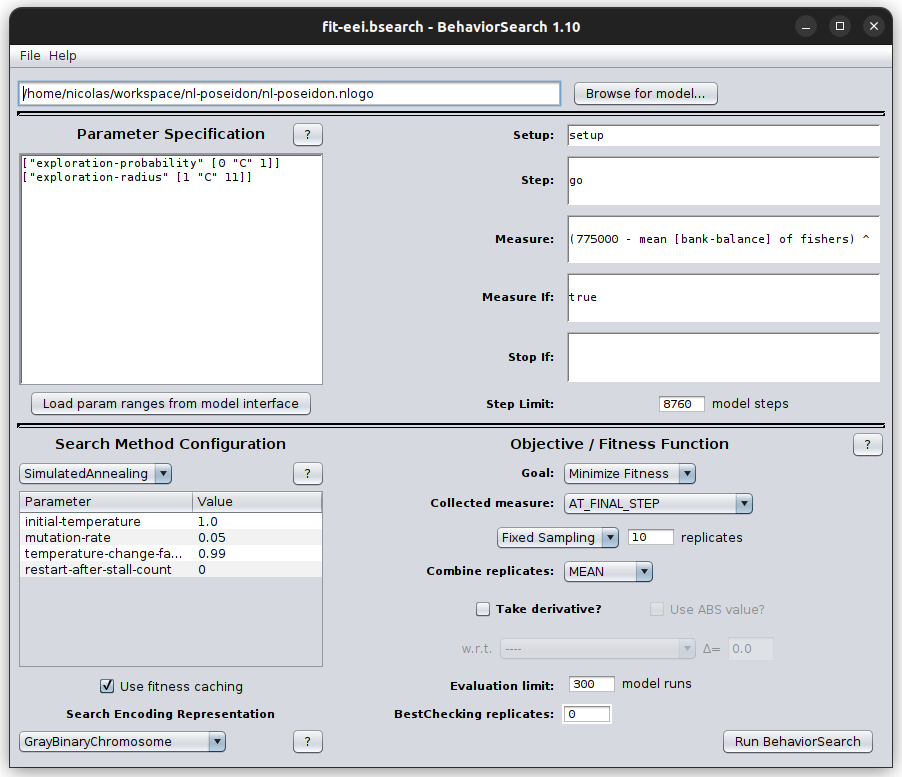
\includegraphics[height=0.8\textheight]{images/bsearch_fit_eei.png}
\end{frame}

\begin{frame}[fragile=singleslide]{Loading BehaviorSearch results automatically}
  \begin{adjustbox}{max height=0.8\textheight, max width = \linewidth}
    \begin{minted}[highlightlines=16-20]{nlogo}  
to load-best [ prefix ]
  let rows csv:from-file word prefix ".finalCheckedBests.csv"
  let headers item 0 rows
  let data first sort-by [ [r1 r2] -> 
    last r1 > last r2 
  ] but-first rows
  foreach range length headers [ i ->
    if last item i headers = "*" [
      let param but-last item i headers
      let value precision item i data 3
      run (word "set " param " " value)
    ]
  ]
end
    \end{minted}
  \end{adjustbox}
\end{frame}

\begin{frame}{Testing sensititivy of EEI parameters}
  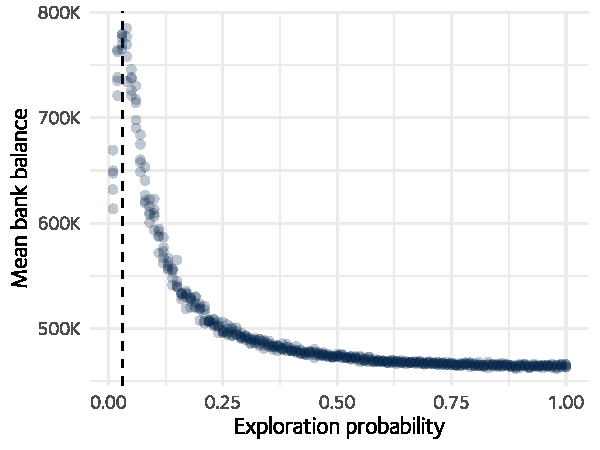
\includegraphics[width=0.49\linewidth]{images/exploration_prob.pdf}
  \hfill
  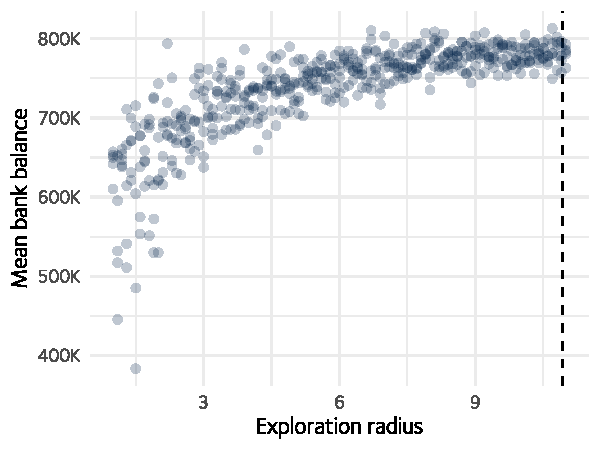
\includegraphics[width=0.49\linewidth]{images/exploration_radius.pdf}
\end{frame}

\begin{frame}{Not looking good for the fishery...}
  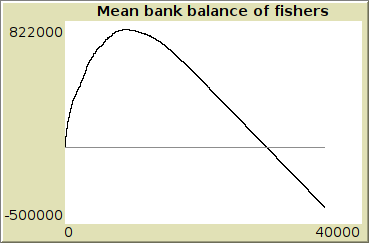
\includegraphics[width=0.49\linewidth]{images/business-as-usual-balance.png}
  \hfill
  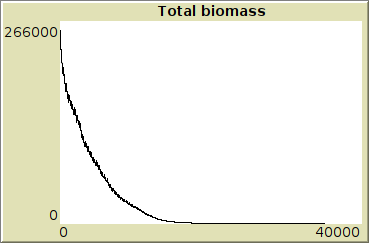
\includegraphics[width=0.49\linewidth]{images/business-as-usual-biomass.png}
\end{frame}

\begin{frame}{Searching for the optimal MPA}
  \centering
  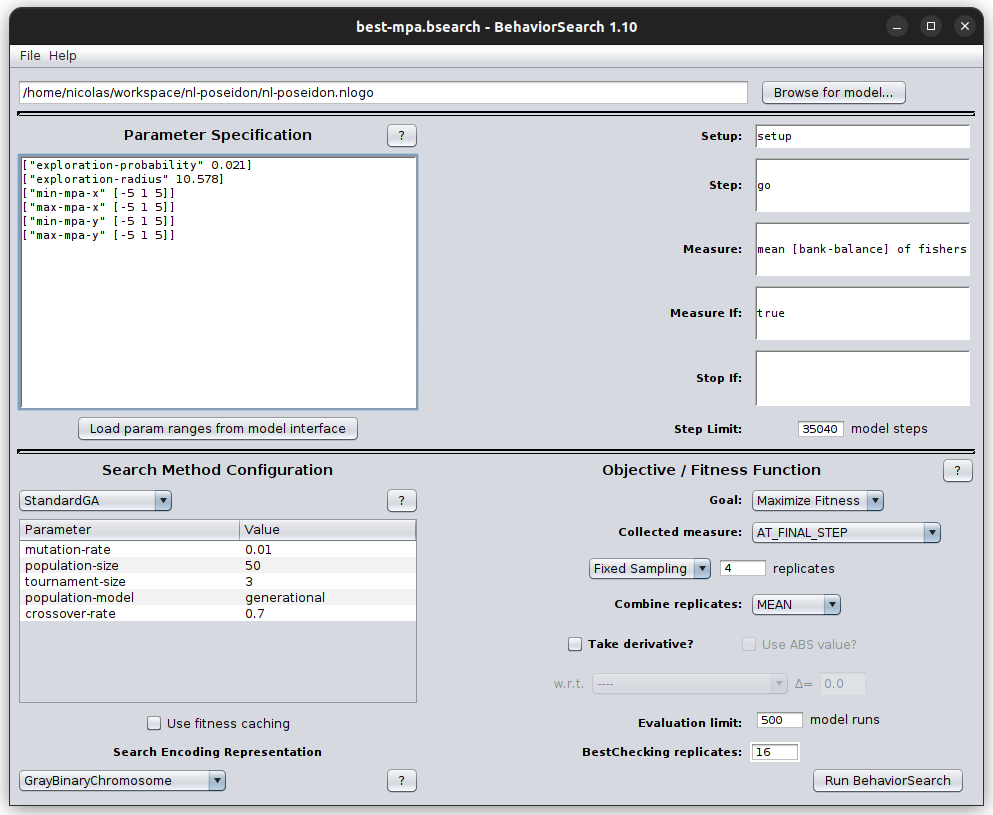
\includegraphics[height=0.8\textheight]{images/bsearch_mpa.png}
\end{frame}

\begin{frame}{Comparing four different scenarios}
  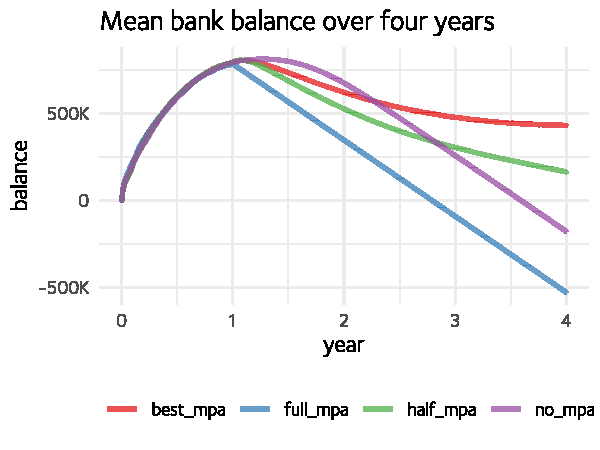
\includegraphics[width=0.49\linewidth]{images/experiment_balance.pdf}
  \hfill
  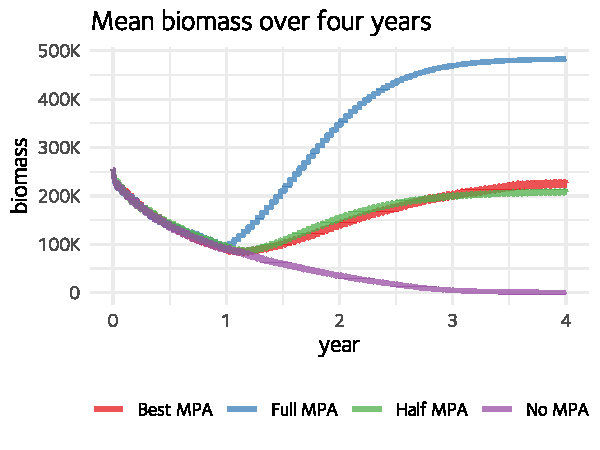
\includegraphics[width=0.49\linewidth]{images/experiment_biomass.pdf}
\end{frame}
